\pagenumbering{arabic} %設定頁號阿拉伯數字
\setcounter{page}{1}  %設定頁數
\section{Starting the simulation 開始模擬}
\subsection{Software option chosen for the simulation模擬所選擇的軟體選項}
\fontsize{14pt}{2.5pt}\sectionef {For this simulation, it has been decided that the best evaluation of the Odoo software would be through its online web-based service. The reasons for such choice instead of using the community edition of the software are as follows:}\\[1pt]
\fontsize{14pt}{5pt}\sectionef{對於這次模擬,我們決定通過Odoo軟體的在線網絡服務來進行最佳評估。選擇這種方式而不是使用軟體的社區版的原因如下:}\\[15pt]

\begin{itemize}
\item The practicality of using a web-based service as oppose to administrate a server locally or remotely. Although the community application was tested as part of the research for this work and has been judged to be a very beginner friendly server application the fact of the matter is that hosting a server is, on its own, a job that requires experience and knowledge. There has been a shift of the market regarding this sort of application towards product as a service and with good reason. At the time this thesis is being written the COVID-19 pandemic is forcing a lot of employees to work remotely and making clear to the market that IT is not a simple job and that a web service is an attractive option.
\item 相對於在本地或遠程管理服務器,使用基於Web的服務的實用性。儘管社區應用程式作為本項研究的一部分進行了測試,並且被判斷為非常適合初學者的服務器應用程式,但實際情況是,單獨運營服務器是一項需要經驗和知識的工作。市場對於這種類型的應用程式發生了轉變,向作為服務的產品轉移,並且有充分的理由。在撰寫本論文時,COVID-19大流行迫使許多員工遠程工作,並向市場表明IT工作並不簡單,而Web服務是一個具有吸引力的選擇。
\vspace{1cm}
\item Lack of official Odoo PLM application for the community edition of Odoo. Although there is a substantial repertoire of community made applications for the community edition of Odoo the organization, description, integration, and support of this applications are spotted at best. Rather than rely on applications that might not keep up with the main software it was decided that it would be a fairer to the platform evaluation if it was based on official applications. I.e. it would be very unproductive to slap together a free solution just to depend on luck regarding how it is supported on the future. PLM is the focus here, so this is an unnegotiable situation.
\item Odoo社區版缺乏官方的Odoo PLM應用程式。儘管有大量的由社區製作的Odoo社區版應用程式,但這些應用程式的組織、描述、整合和支持最多也只是達到及格水平。與其依賴可能跟不上主要軟體步伐的應用程式,我們決定,如果基於官方應用程式進行評估,將更公平地評估該平台。換句話說,將一個免費解決方案隨便拼湊在一起,僅僅依靠未來它如何得到支持,是非常不划算的。在這裡PLM是重點,因此這是一個不可妥協的情況。
\end{itemize}

\newpage
\fontsize{14pt}{2.5pt}\sectionef {At the time of writing this work, Odoo allows you to select one of its extra features like PLM and use it for free for an indefinite amount of time on their cloud hosted servers. This is a very attractive option if the only focus of this work was PLM and manufacturing. However, the MES aspect of this work is highly dependent of other applications of Odoo which means that there is very little that can be done. To this end the experiment was carried out in the trial version of Odoo enterprise which allow the user to use the system without storage or application limitations for a period of 14 days all hosted in Odoo cloud servers (Figure 17).}\\[1pt]
\fontsize{14pt}{5pt}\sectionef{在撰寫本文時,Odoo允許您在其雲端主機上選擇其額外功能之一,例如PLM,並無限期免費使用。如果本文的唯一焦點是PLM和製造業,那麼這是一個非常吸引人的選擇。然而,這項工作的MES方面高度依賴Odoo的其他應用程式,這意味著幾乎沒有什麼可以做。因此,實驗是在Odoo企業版的試用版本中進行的,該版本允許用戶在Odoo雲端服務器上使用系統,沒有存儲或應用程式限制,使用期限為14天(圖17)。}\\[15pt]
\subsection{Setings details that are relevant相關的設置細節}
\fontsize{14pt}{2.5pt}\sectionef {A few details regarding the settings of Odoo are relevant to the proper function of its manufacturing functionalities. Namely enabling work orders in the manufacturing settings is an obligatory step for proper use of both work order items, workcenter items and operation items.}\\[1pt]
\fontsize{14pt}{5pt}\sectionef{關於Odoo設置的一些細節與其製造功能的正確運作相關。具體而言,啟用製造設置中的工單是使用工單項目、工作中心項目和操作項目的正確步驟。}\\[15pt]
\fontsize{14pt}{2.5pt}\sectionef {An assumption made for this work is that this is a holdover of the ERP origins of the software because it is rather unintuitive to not have this setting enabled by default if you are going to use Odoo to make any serious control on manufacturing. Regardless as of Odoo enterprise v14 this option can be set in the Settings > Manufacturing > Operations > Work Orders (Figure 28).}\\[1pt]
\fontsize{14pt}{5pt}\sectionef{這項工作的假設是,這是該軟件的ERP起源的遺留問題,因為如果您要在Odoo上進行任何嚴肅的製造控制,那麼不將此設置默認啟用是相當不直觀的。儘管如此,從Odoo企業版v14開始,可以在「設置」>「製造」>「操作」>「工單」中設置此選項(圖28)。}\\[15pt]
\newpage

\begin{figure}[hbt!]
\begin{center}
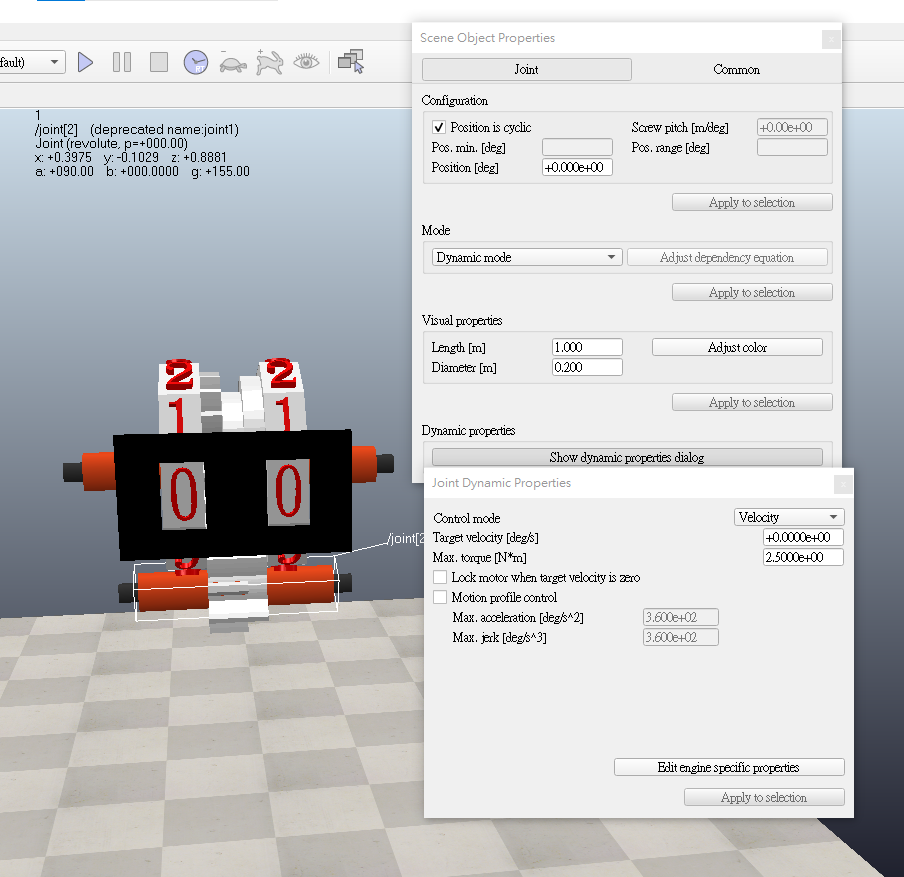
\includegraphics[width=15cm]{28}
\caption{\large Screenshot of the specific setting to be enabled\\特定設置的截圖}\label{fig.28}
\end{center}
\end{figure}

\section{Building the company structure 建立公司結構}
\subsection{User 使用者}

\fontsize{14pt}{2.5pt}\sectionef {Users are set and invited through the setting menu. It is possible to assign different levels of permissions regarding different aspects of the business operation. Messaging, permissions,approvals, responsibilities are all assigned into a user. This is very convenient and can fall within the category of virtual item class even if it has limited use in the scope of manufacturing. Their creation is not strictly necessary, the software would run just fine having just me as a user with full administrator credentials, but for this simulation, 5 users were created as listed below to represent different employees within the company. The following (Figure 29) is a screenshot of my user account item and its ‘Asses Rights’ followed by one of the fictional users being created for the company (Figure 30).}\\[1pt]
\fontsize{14pt}{5pt}\sectionef{使用者是透過設置選單設定並邀請的。可以針對業務運作的不同方面分配不同級別的權限。訊息、權限、批准、責任等都分配給使用者。這非常方便,即使在製造範圍內使用有限,也可以歸入虛擬項目類別。它們的創建不是絕對必要的,軟體只需我作為具有完整管理員權限的使用者即可正常運行,但為了這個模擬,已創建了5個使用者,如下所列,代表公司內的不同員工。下面(圖29)是我的使用者帳戶項目及其“評估權限”,接著是為公司創建的虛構使用者之一(圖30)的截圖。}\\[15pt]
\newpage

\begin{figure}[hbt!]
\begin{center}
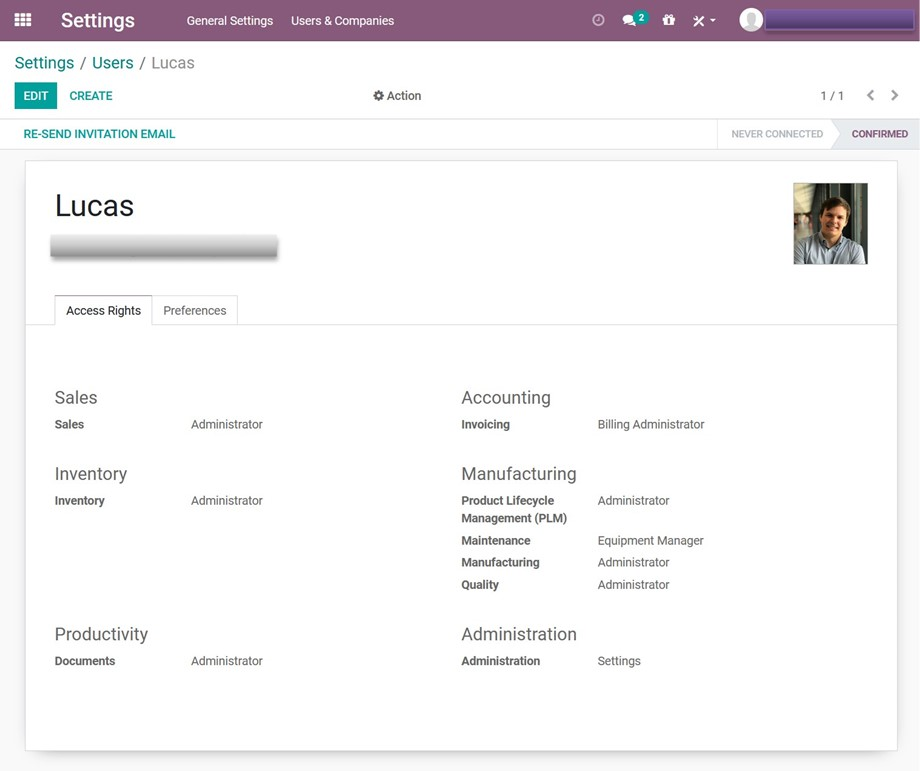
\includegraphics[width=15cm]{29}
\caption{\large  Screenshot of user account interface\\使用者帳戶介面截圖}\label{fig.29}
\end{center}
\end{figure}
\newpage

\begin{figure}[hbt!]
\begin{center}
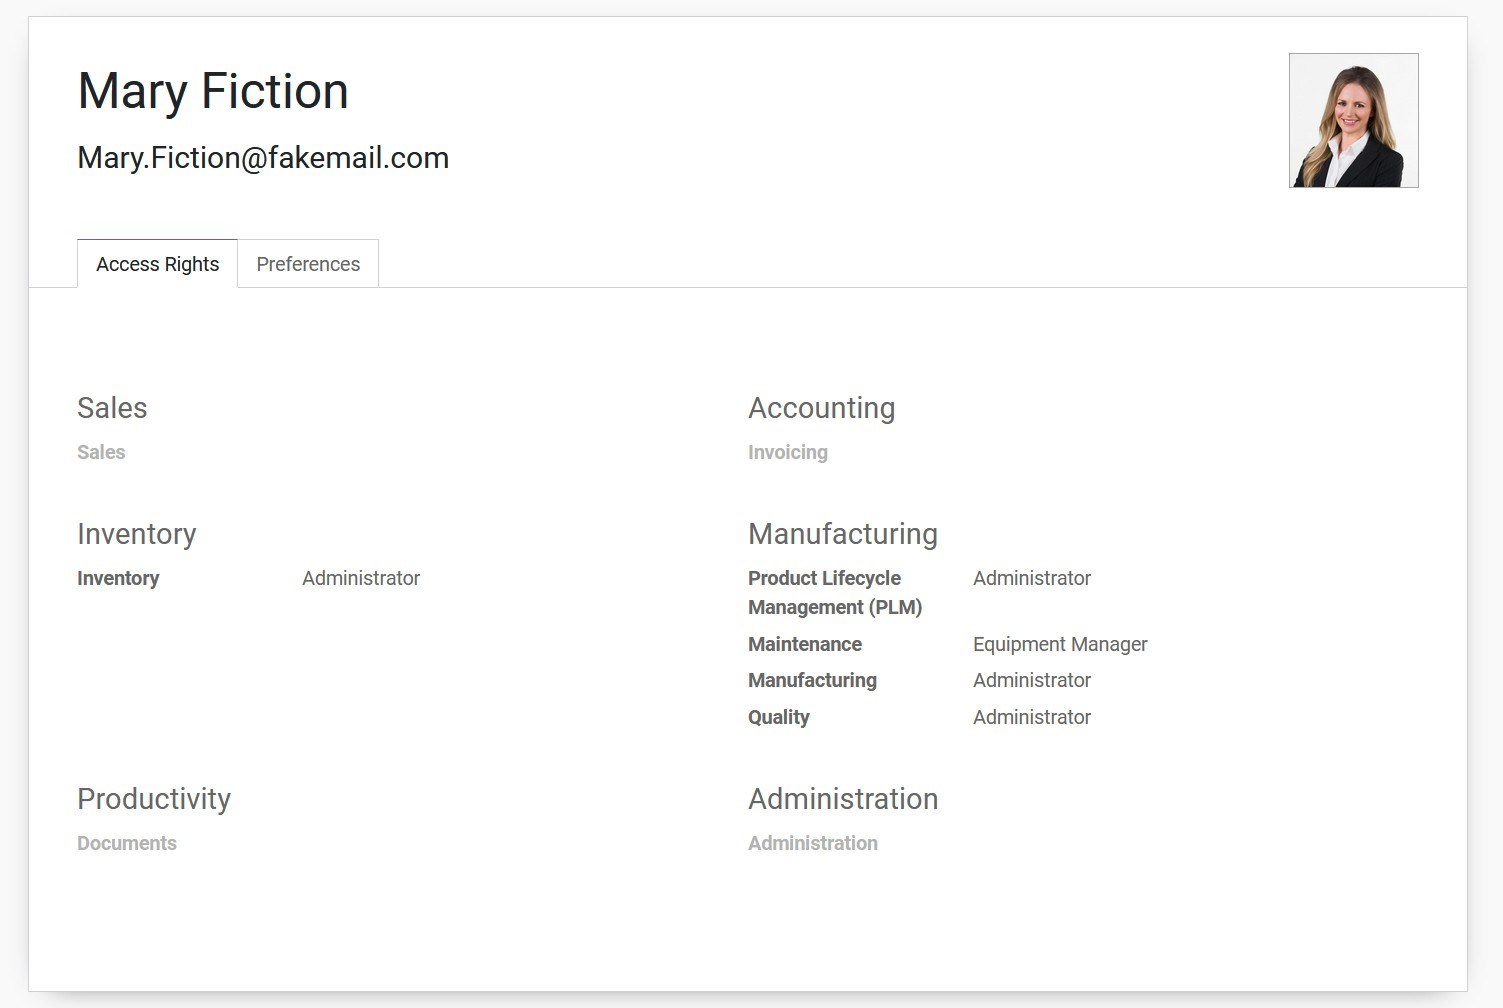
\includegraphics[width=15cm]{30}
\caption{\large  Screenshot of second user account interface\\第二個使用者帳戶介面截圖}\label{fig.30}
\end{center}
\end{figure}

\fontsize{14pt}{2.5pt}\sectionef {It is nice to point out how the two differ in access rights. Mary Fiction has been created in this example as an engineer and therefore most of her permissions are around the manufacturing procedure while she is denied access to other parts like Sales or Accounting.}\\[1pt]
\fontsize{14pt}{5pt}\sectionef{很好地指出這兩個使用者在訪問權限上的差異是不錯的。在這個例子中,Mary Fiction 被創建為一名工程師,因此她的大部分權限都圍繞著製造程序,同時她被拒絕訪問其他部分,如銷售或會計。}\\[15pt]

\subsection{Workcenters and Equipement 工作中心和設備}
\fontsize{14pt}{2.5pt}\sectionef {Workcenters are quite flexible within Odoo in the sense that they can be changed and expanded as needed. One could create the workcenters after creating the product items to allow for reorganization of the shop floor once you gained some perspective on what the products will be in the end. However, for most scenarios this seems unrealistic since the workcenters are more rigid structures in the real world - they don’t change as much as the products since they tend to hold heavy machinery.}\\[1pt]
\fontsize{14pt}{5pt}\sectionef{在Odoo中,工作中心在某種程度上非常靈活,可以根據需要進行更改和擴展。您可以在創建產品項目之後創建工作中心,以便在獲得一些關於最終產品的想法後重新組織車間。然而,對於大多數情況來說,這似乎不太現實,因為工作中心在現實世界中更加固定 - 它們不像產品那樣經常變化,因為它們往往安裝有重型機械。}\\[15pt]
\newpage

\fontsize{14pt}{2.5pt}\sectionef {In this simulation it was considered that the company already has 3 workcenters from the get-go and therefore the workcenters and machinery were created beforehand. This is more useful for possible readers interested in implementing Odoo as well as saving sometime.}\\[1pt]
\fontsize{14pt}{5pt}\sectionef{在這個模擬中,考慮到公司從一開始就已經擁有了3個工作中心,因此工作中心和機械是事先創建的。這對於有興趣實施Odoo的潛在讀者來說更加有用,也可以節省時間。}\\[15pt]

\fontsize{14pt}{2.5pt}\sectionef {We begin by creating the equipment we have. This is an item class that emphasizes in maintenance organization. The application responsible for managing equipment is the Maintenance App. The following image is an example of how Odoo portrays a 3D printer equipment item (Figure 31).}\\[1pt]
\fontsize{14pt}{5pt}\sectionef{我們首先創建我們擁有的設備。這是一個強調維護組織的項目類別。負責管理設備的應用程序是維護應用。下面的圖像是Odoo展示一個3D打印機設備項目的示例(圖31)。}\\[15pt]
\begin{figure}[hbt!]
\begin{center}
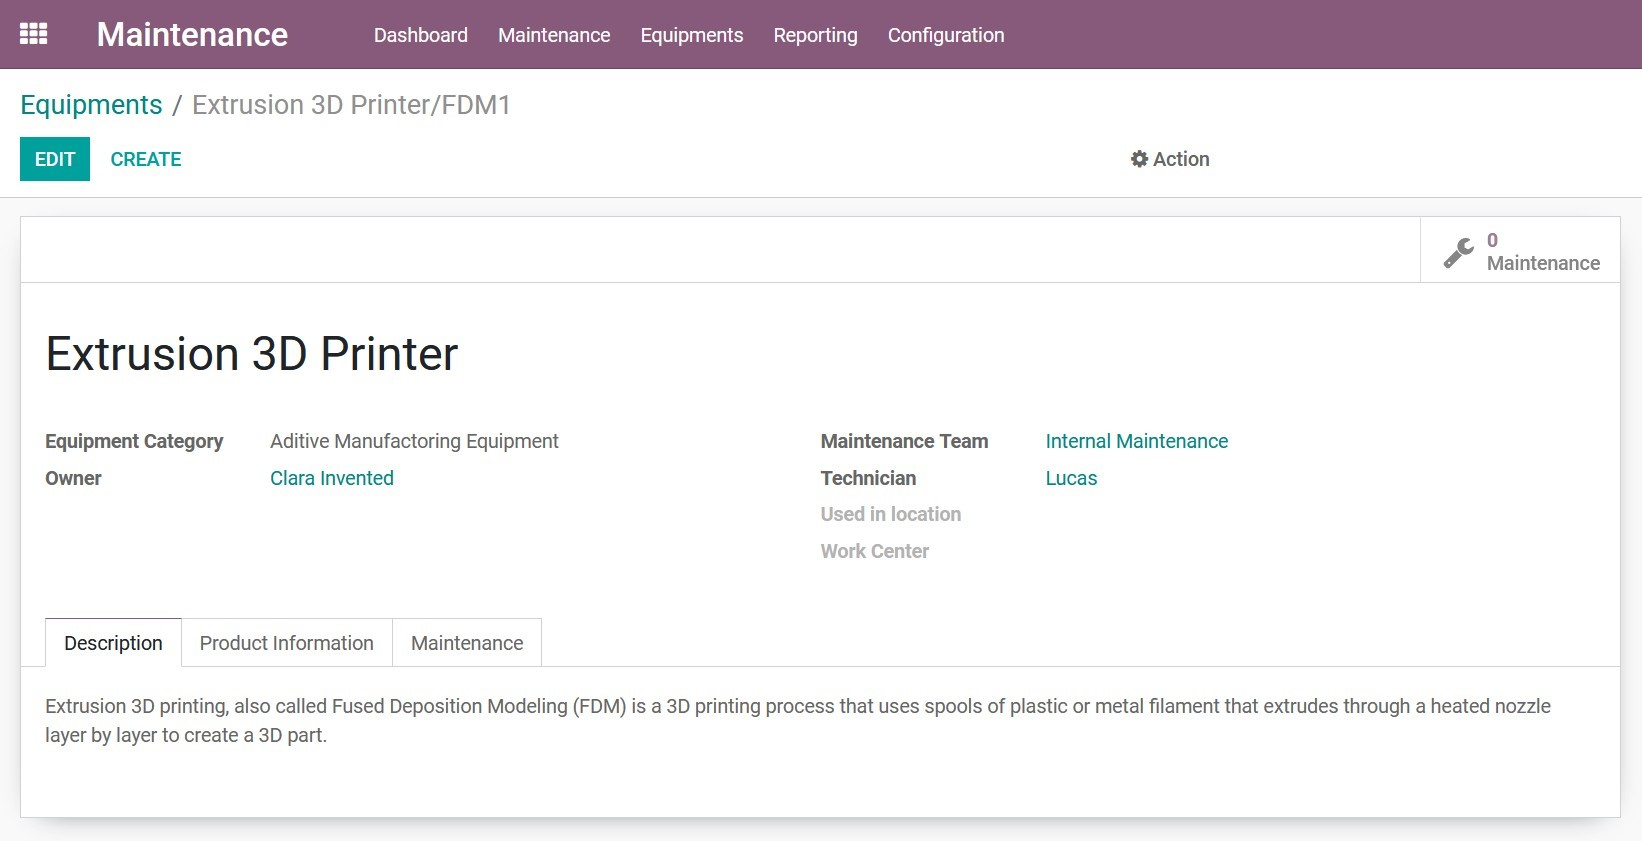
\includegraphics[width=15cm]{31}
\caption{\large  Odoo 3D printer equipment item\\Odoo 3D打印機設備項目}\label{fig.31}
\end{center}
\end{figure}

\fontsize{14pt}{2.5pt}\sectionef {In addition to this 3D printer the following equipment were created to be used throughout the development/production process (Figure 32):}\\[1pt]
\fontsize{14pt}{5pt}\sectionef{除了這台3D打印機外,還創建了以下設備,用於整個開發/生產過程}\\[15pt]
\fontsize{14pt}{5pt}\sectionef{(圖32):}\\[15pt]
\newpage

\begin{figure}[hbt!]
\begin{center}
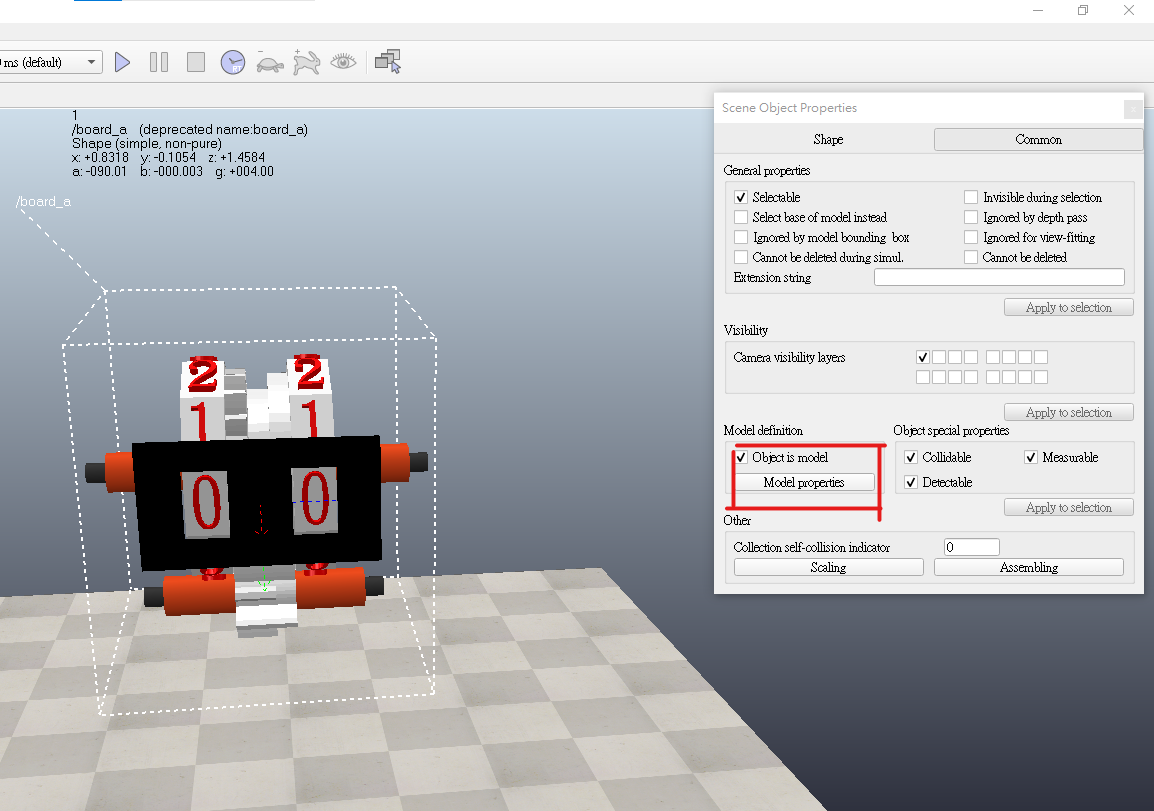
\includegraphics[width=15cm]{32}
\caption{\large  Overview of equipment items\\設備項目概觀}\label{fig.32}
\end{center}
\end{figure}

\fontsize{14pt}{2.5pt}\sectionef {This is where software limitations regarding PLM start to show. Although equipment items allow you some level of metadata (description text, responsible user, maintenance data and vendor). It does not allow for the uploading of files of any kind to be attached to the item class (machine manuals, reports etc). This is a substantial weakness, since file management is something quite unanimously considered a main aspect of PLM. This will be a recurring subject of this simulation since the number of Items that allow upload of files directly to them is limited in Odoo.}\\[1pt]
\fontsize{14pt}{5pt}\sectionef{這就是軟件在產品生命週期管理(PLM)方面開始顯示限制的地方。儘管設備項目允許一定程度的元數據(描述文字、負責用戶、維護數據和供應商),但它不允許上傳任何類型的文件附加到項目類別(機器手冊、報告等)。這是一個相當大的弱點,因為文件管理被普遍認為是PLM的主要方面之一。這將是這次模擬的一個反復出現的主題,因為在Odoo中,允許直接上傳文件的項目數量是有限的。}\\[15pt]
\fontsize{14pt}{2.5pt}\sectionef {Now that the equipment has been created, their workcenters can be created. It is interesting to remember that the main use of the workcenter item is management of time and cost per hour. The idea is that equipment assigned to a WC should not be used at the same time and that ideally equipment that have widely different running costs should also be in different workcenters to allow for better time/cost tracking.}\\[1pt]
\fontsize{14pt}{5pt}\sectionef{現在設備已經創建,它們的工作中心可以被建立了。值得一提的是,工作中心項目的主要用途是按小時管理時間和成本。這個想法是分配給工作中心的設備不應該同時使用,而且理想情況下,具有截然不同的運行成本的設備也應該位於不同的工作中心,以便更好地跟蹤時間/成本。}\\[15pt]
\fontsize{14pt}{2.5pt}\sectionef {The following (Figure 33) is a an example of a workcenter item made to represent the prototyping station that is used throughout the development of the product.}\\[1pt]
\fontsize{14pt}{5pt}\sectionef{以下(圖33)是一個工作中心項目的示例,用來代表在產品開發過程中使用的原型製作站。}\\[15pt]
\newpage

\begin{figure}[hbt!]
\begin{center}
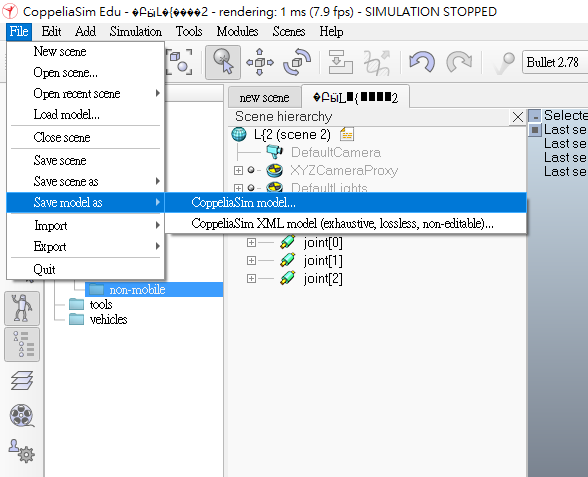
\includegraphics[width=15cm]{33}
\caption{\large  Odoo Prototyping Station item representation 1\\Odoo原型製作站項目表示1}\label{fig.33}
\end{center}
\end{figure}

\fontsize{14pt}{2.5pt}\sectionef {The reader will notice that this station (Figure 34) is where the 3D printers and CNC machine are located. Usually these machines would be separated in singular workcenters because of difference in operation costs and because they are for the most part independent however for the sake of this simulation this has been considered representative enough.}\\[1pt]
\fontsize{14pt}{5pt}\sectionef{讀者會注意到這個站點(圖34)是3D打印機和CNC機床的所在地。通常,由於操作成本的差異以及它們在很大程度上是獨立的,這些機器會被分開放置在不同的工作中心中。然而,出於模擬的目的,這被認為足夠具有代表性}\\[15pt]
\newpage

\begin{figure}[hbt!]
\begin{center}
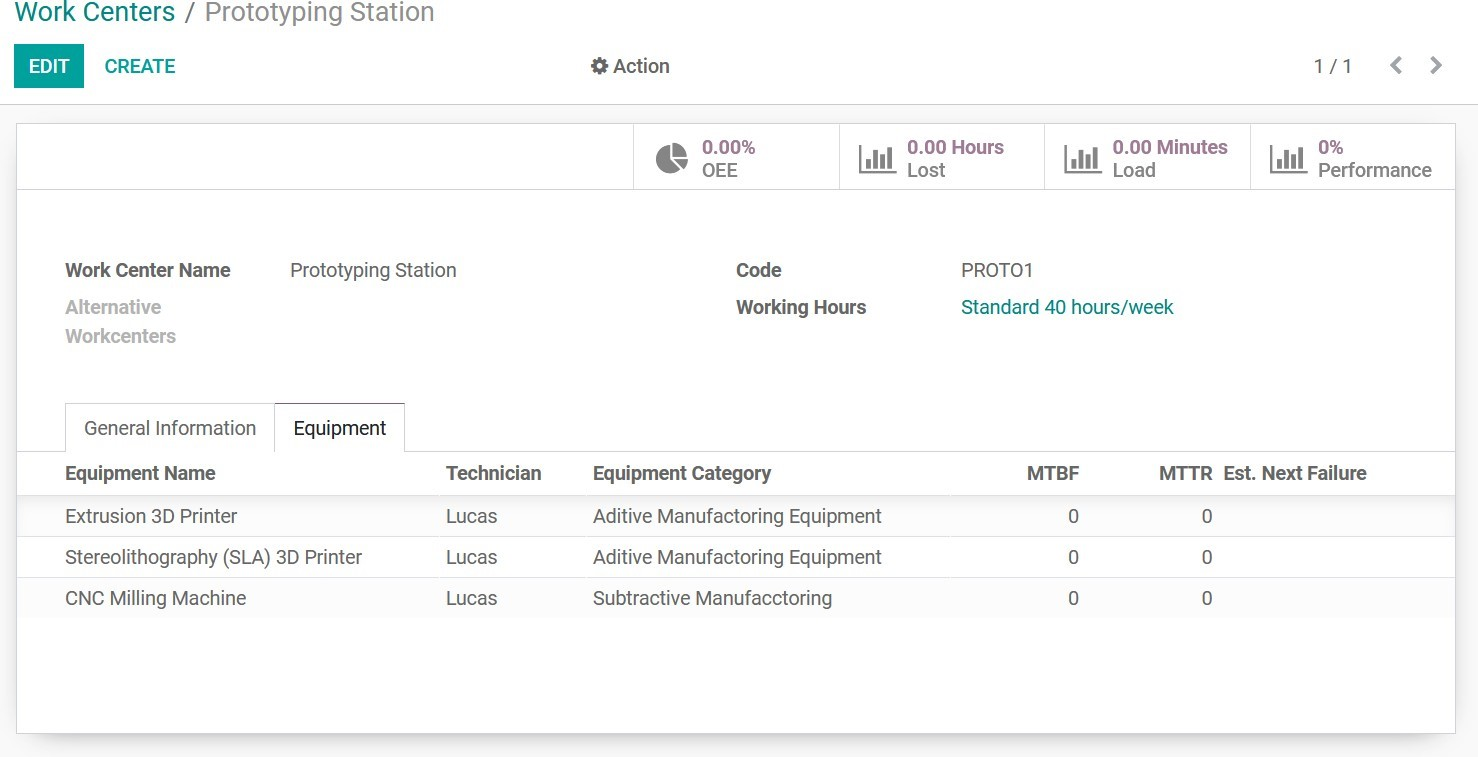
\includegraphics[width=15cm]{34}
\caption{\large  Prototyping Station item representation 2\\原型製作站項目表示2}\label{fig.34}
\end{center}
\end{figure}

\fontsize{14pt}{2.5pt}\sectionef {The following (Figure 35) workcenters have been also created for the simulation and filed with the necessary equipment:}\\[1pt]
\fontsize{14pt}{5pt}\sectionef{以下(圖35)工作中心也已經為模擬創建並填入必要的設備:}\\[15pt]

\begin{figure}[hbt!]
\begin{center}
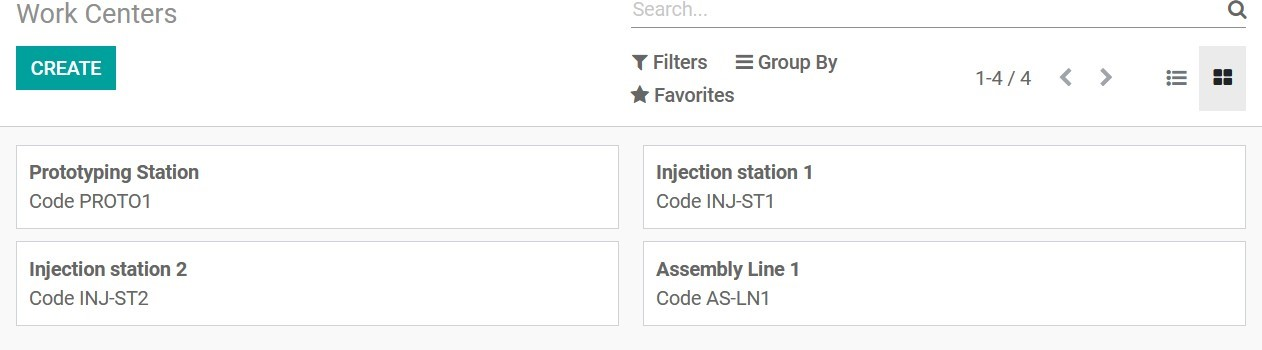
\includegraphics[width=15cm]{35}
\caption{\large  Overview of Workcenter items\\工作中心項目概覽}\label{fig.35}
\end{center}
\end{figure}